\documentclass[a4paper,12pt]{article}

\usepackage[utf8]{inputenc}
\usepackage[T1]{fontenc}
\usepackage[french]{babel}
\usepackage{geometry}
\usepackage{amsmath,amssymb}
\usepackage{graphicx}
\usepackage{float}
\usepackage{booktabs}
\usepackage{array}
\usepackage{hyperref}
\usepackage{setspace}
\usepackage{enumitem}
\usepackage{xcolor}
\usepackage{pdfpages}
\usepackage{titling}

\geometry{margin=2.5cm}

\title{\textbf{Prédiction du prix des logements à Boston par régression linéaire}}
\author{Dalikan N'guessan}
\date{\today}

\begin{document}

\maketitle

\begin{abstract}
Le projet consiste à prédire la valeur médiane des logements à Boston à partir de variables socio-économiques et urbaines, en utilisant un modèle de régression linéaire multiple. Le jeu de données contient 506 observations et 13 variables explicatives, ainsi qu’une variable cible continue. Après séparation aléatoire en ensemble d’entraînement et de test, le modèle est estimé par moindres carrés ordinaires. Les résultats montrent un ajustement satisfaisant : le coefficient de détermination est de 0,7509 sur les données d’entraînement et de 0,6688 sur les données de test. Le RMSE est de 4,65 milliers de dollars en apprentissage et de 4,93 milliers de dollars en test. Les diagnostics indiquent que le modèle capture bien l’essentiel de la structure de la donnée, mais que les hypothèses d’homoscédasticité et de normalité des résidus ne sont pas totalement respectées. Cette étude permet ainsi de tester une chaîne complète de travail en data science : exploration, modélisation, évaluation et diagnostic critique.

\textbf{Mots-clés : } régression linéaire, Boston Housing, analyse exploratoire, diagnostics du modèle, machine learning.
\end{abstract}

\tableofcontents
\newpage

\section{Introduction}

Le jeu de données Boston Housing est un exemple classique de problème de prédiction immobilière. Il décrit plusieurs quartiers de Boston au début des années 1970 et contient des informations sur la démographie, la qualité de l’environnement, l’accès aux services et les caractéristiques socio-économiques. L’objectif est d’expliquer la variable cible, la valeur médiane des logements, à partir d’un ensemble de variables explicatives.

Cette étude s’inscrit dans une logique de montée en compétence en data science. L’enjeu n’est pas seulement d’obtenir un bon score, mais surtout de maîtriser les étapes essentielles d’un projet de modélisation : nettoyage des données, analyse exploratoire, validation, interprétation et diagnostic des hypothèses. La régression linéaire est utilisée ici comme modèle de référence, car elle reste un outil simple, explicable et très utile pour comprendre les relations entre variables.

Le rapport est organisé comme suit : la section 2 présente les données et l’analyse exploratoire, la section 3 décrit la méthodologie, la section 4 expose les résultats, la section 5 analyse les hypothèses du modèle, puis la section 6 conclut la discussion et les perspectives.

\section{Données et analyse exploratoire}

\subsection{Présentation du jeu de données}
Le jeu de données comprend 506 observations et 14 variables numériques, dont 13 variables explicatives et une variable cible : \textit{Valeur\_med\_logement}. Les différentes colonnes décrivent notamment la criminalité, la proportion de terrains résidentiels, la densité industrielle, la proximité des centres d’emploi, le nombre de pièces, la proportion de logements anciens, l’impôt foncier, le taux de population défavorisée, ainsi que l’accès aux autoroutes.

Les données ne comportent pas de valeurs manquantes. Les colonnes ont été renommées pour améliorer la lisibilité du notebook et du rapport.

\begin{table}[H]
\centering
\caption{Description des variables du jeu de données}
\begin{tabular}{lp{9cm}}
\toprule
Variable & Description \\
\midrule
Taux\_criminalite & Taux de criminalité par habitant \\
Prop\_terrains\_resid & Proportion de terrains résidentiels en lots de plus de 25 000 pieds carrés \\
Prop\_acres\_indus & Proportion de surface industrielle \\
Bordure\_riviere & Variable binaire indiquant si le quartier borde la rivière \\
Concentration\_NO2 & Concentration de dioxyde d’azote \\
Nb\_pieces\_logement & Nombre moyen de pièces par logement \\
Prop\_log\_construits\_av1940 & Proportion de logements construits avant 1940 \\
Dist\_ponderees\_emploi & Distance pondérée aux centres d’emploi \\
Accessibilite\_autoroute & Indice d’accessibilité aux autoroutes \\
Taux\_impot\_foncier & Taux d’impôt foncier \\
Ratio\_eleve\_prof & Ratio élèves-professeurs \\
Prop\_noirs\_ville & Proportion de population noire \\
Pourcentage\_pop\_inf & Pourcentage de population défavorisée \\
Valeur\_med\_logement & Valeur médiane des logements (cible) \\
\bottomrule
\end{tabular}
\end{table}

\subsection{Analyse exploratoire}
L’analyse exploratoire a mis en évidence des distributions hétérogènes pour plusieurs variables. Les histogrammes et les boxplots montrent notamment une forte asymétrie pour des variables comme le taux de criminalité et la proportion de population défavorisée. Les variables les plus liées à la cible sont le nombre de pièces, la distance aux centres d’emploi et le pourcentage de population défavorisée.

\begin{figure}[H]
\centering
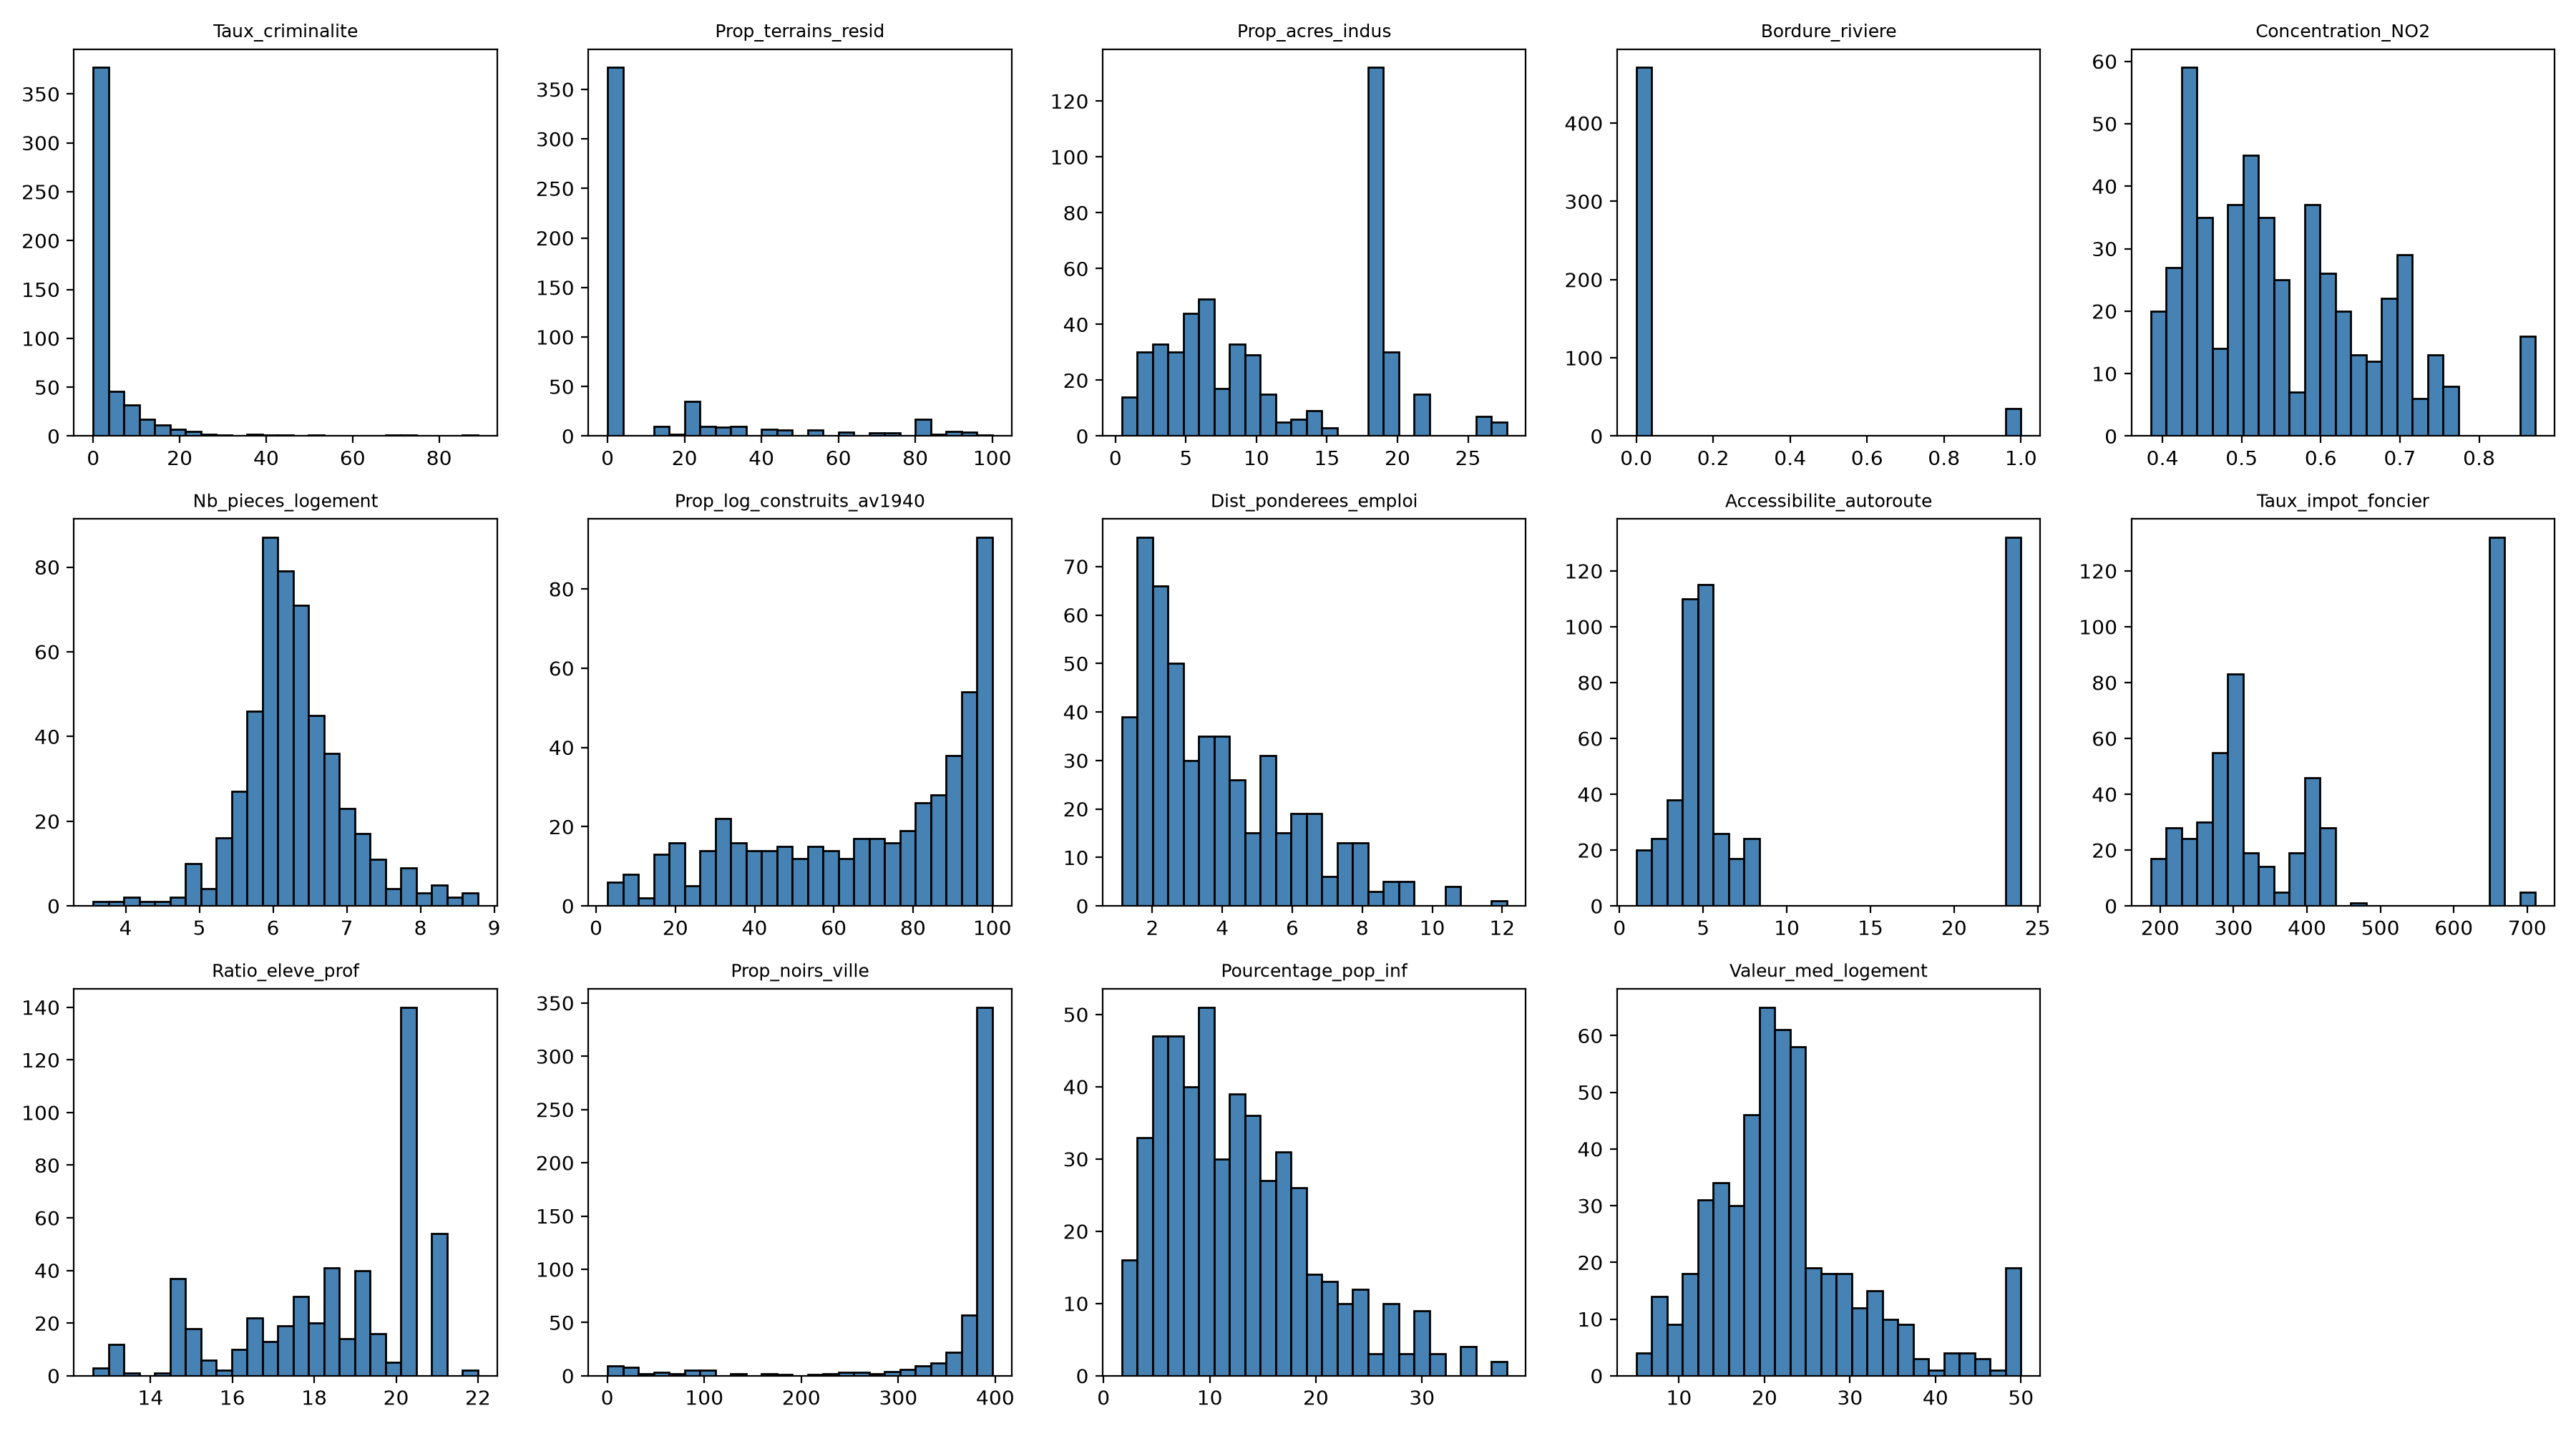
\includegraphics[width=0.96\textwidth]{images/histogrammes.png}
\caption{Histogrammes des variables du jeu de données}
\end{figure}

\begin{figure}[H]
\centering
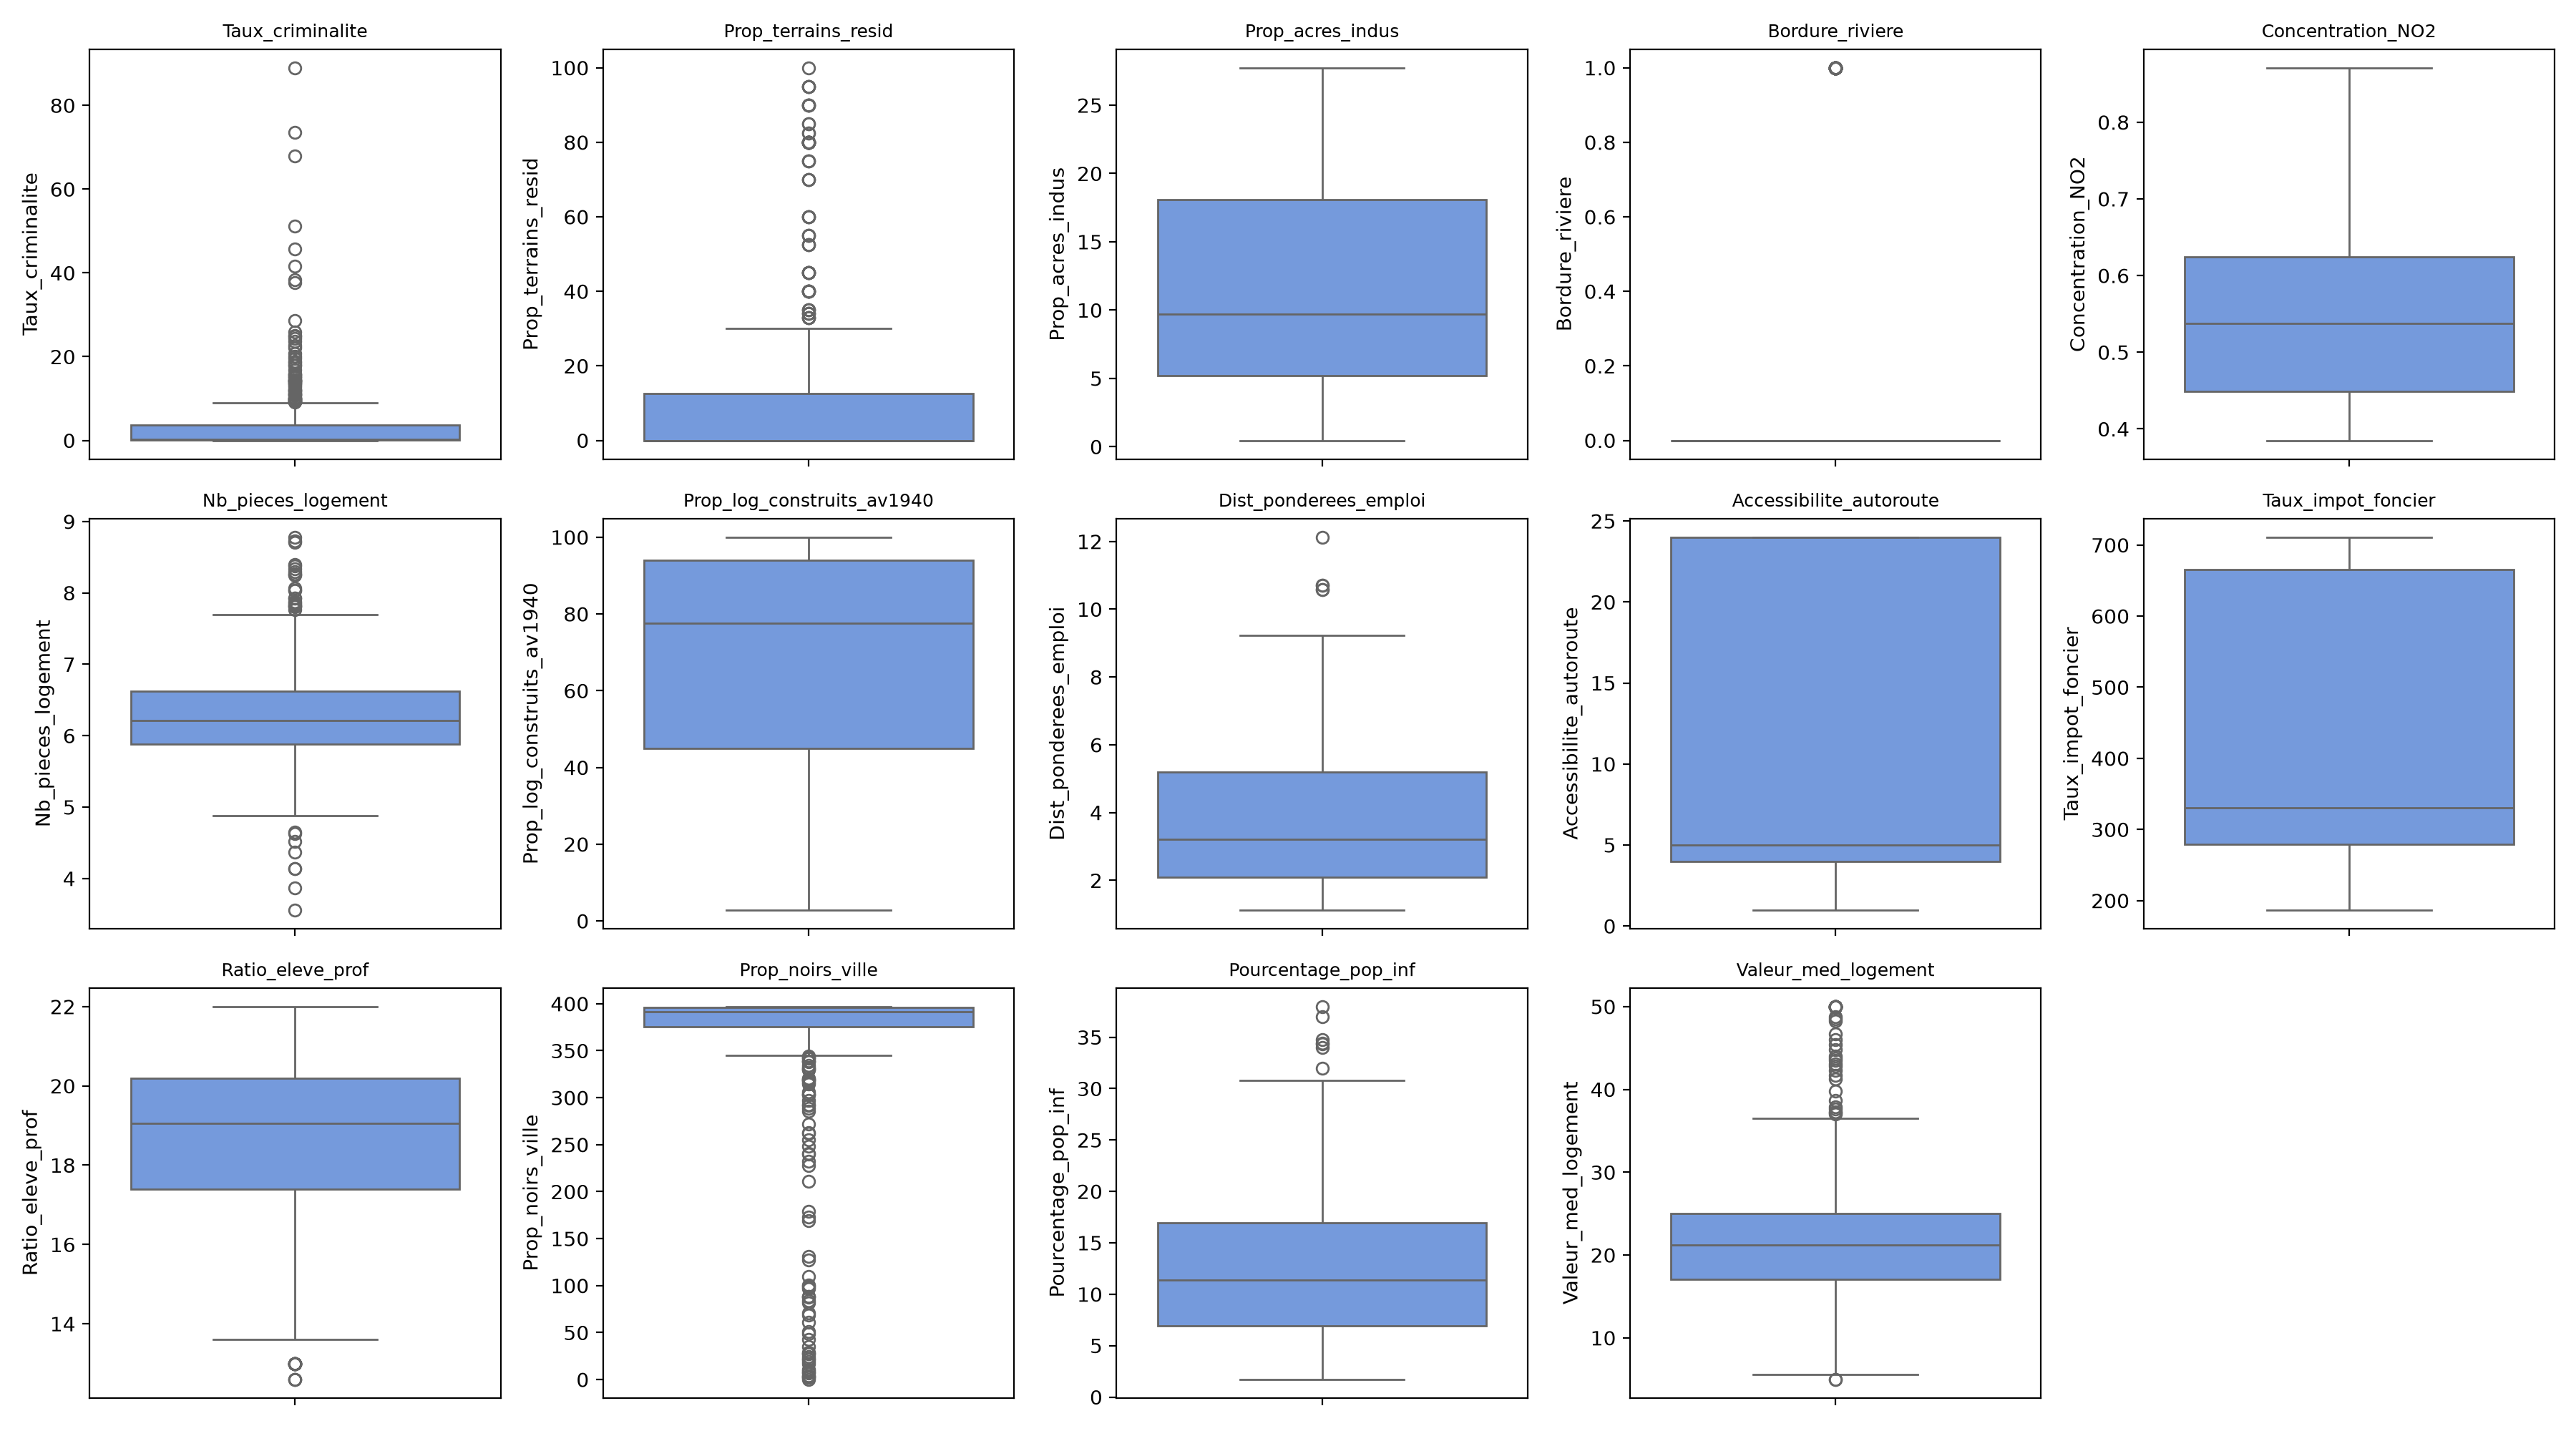
\includegraphics[width=0.96\textwidth]{images/boxplots.png}
\caption{Boxplots des variables explicatives}
\end{figure}

\begin{figure}[H]
\centering
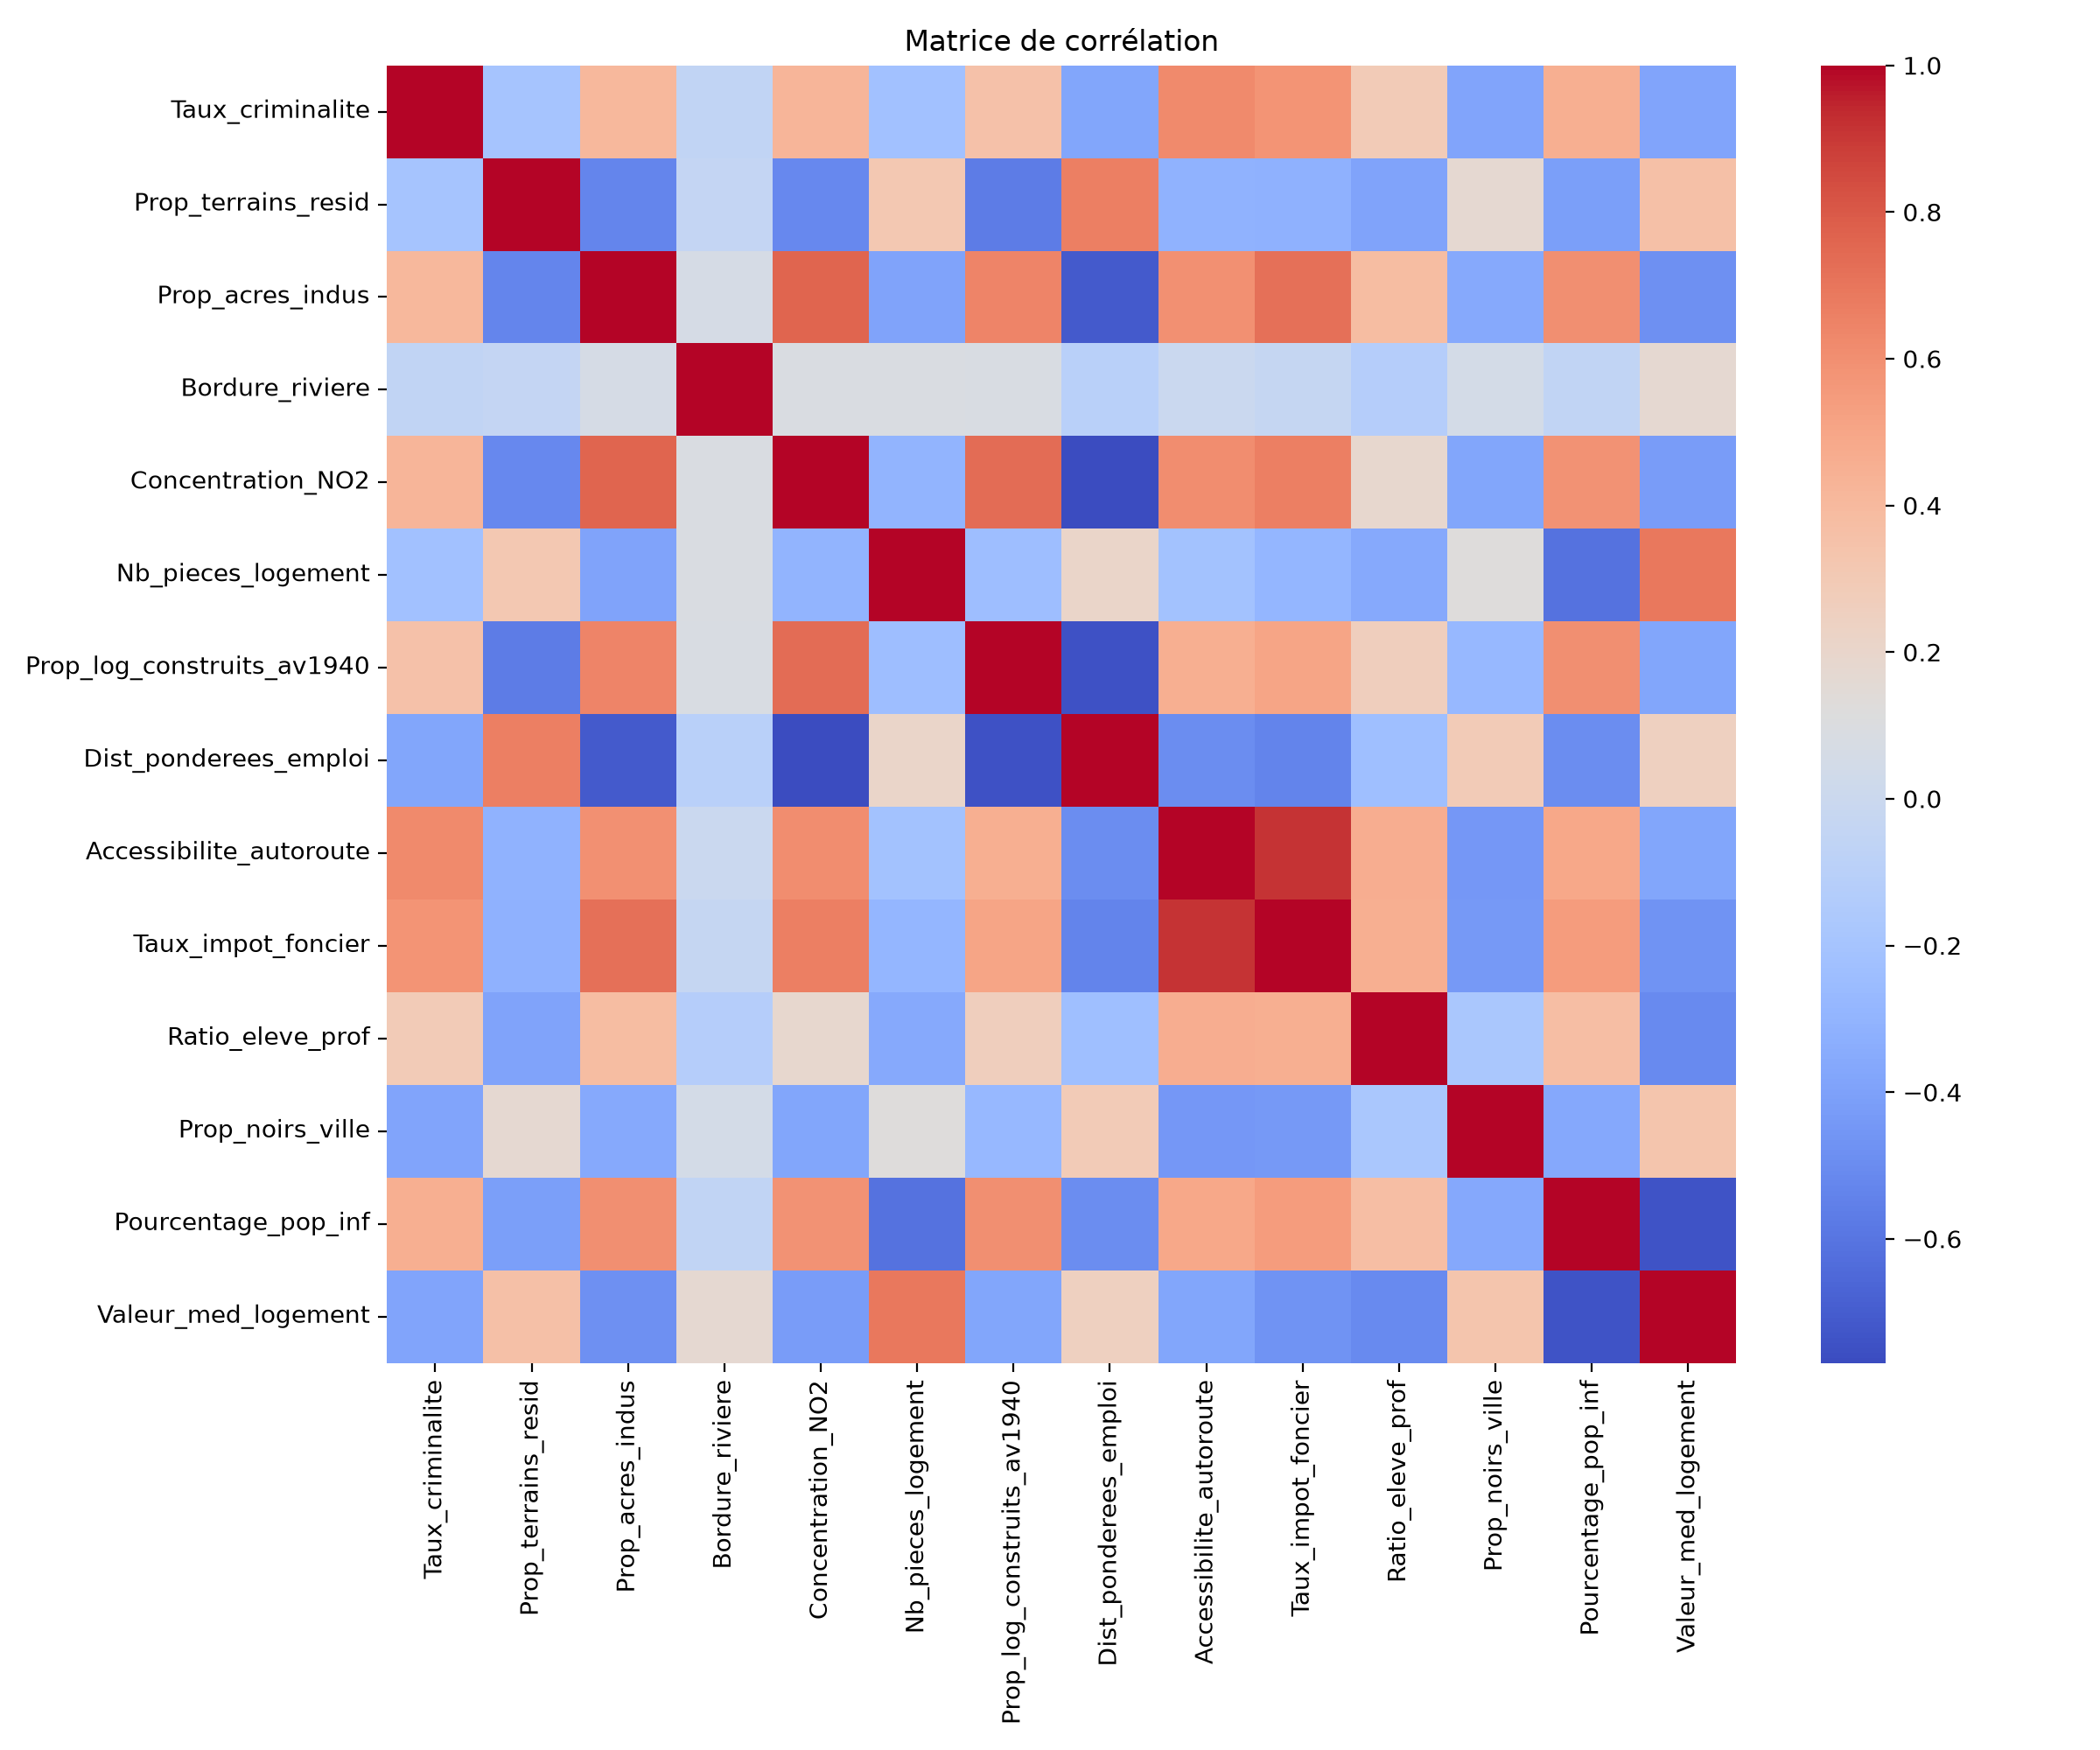
\includegraphics[width=0.9\textwidth]{images/heatmap_correlation.png}
\caption{Matrice de corrélation entre variables}
\end{figure}

Les nuages de points confirment la présence d’une relation marquée entre la valeur du logement et les variables les plus corrélées à la cible. La corrélation la plus forte en valeur absolue est observée pour le nombre de pièces, tandis que le pourcentage de population défavorisée est associé à une baisse de la valeur des logements. La matrice de corrélation montre aussi qu’il existe des couples de variables fortement corrélés, notamment entre l’accessibilité aux autoroutes et le taux d’impôt foncier, ce qui justifie la surveillance de la multicolinéarité.

\subsection{Séparation train-test}
Les données sont divisées en deux sous-ensembles : 80\% pour l’entraînement et 20\% pour le test, avec un paramètre aléatoire fixé à 42 afin d’assurer la reproductibilité. Le jeu de test n’est utilisé qu’à la fin pour évaluer la généralisation du modèle.

\subsection{Modèle de régression linéaire}
Le modèle estimé est une régression linéaire multiple, de la forme :

\[
Y = \beta_0 + \beta_1 X_1 + \beta_2 X_2 + \cdots + \beta_{13} X_{13} + \varepsilon
\]

Les coefficients sont estimés par la méthode des moindres carrés ordinaires (OLS) avec la bibliothèque \texttt{statsmodels}. Le modèle comprend une constante ainsi que les 13 variables explicatives. Aucune transformation ni normalisation particulière n’est appliquée aux variables avant l’ajustement.

\subsection{Métriques d’évaluation}
La performance du modèle est évaluée avec les métriques suivantes :

\begin{itemize}[leftmargin=1.5em]
    \item coefficient de détermination $R^2$ ;
    \item erreur quadratique moyenne (MSE) ;
    \item racine carrée de l’erreur quadratique moyenne (RMSE).
\end{itemize}

Ces métriques sont calculées à la fois sur les données d’entraînement et sur les données de test afin d’évaluer le niveau d’ajustement et la capacité de généralisation.

\subsection{Diagnostics du modèle}
Les hypothèses du modèle sont vérifiées grâce à plusieurs outils :

\begin{itemize}[leftmargin=1.5em]
    \item diagramme des résidus contre les prédictions ;
    \item test de Breusch-Pagan pour l’hétéroscédasticité ;
    \item facteur d’inflation de la variance (VIF) pour la multicolinéarité ;
    \item histogramme et QQ-plot des résidus pour la normalité ;
    \item test de Durbin-Watson pour l’autocorrélation.
\end{itemize}

\section{Résultats}

\subsection{Performance du modèle}
Les résultats du modèle sur les données d’entraînement et de test sont présentés dans le tableau ci-dessous.

\begin{table}[H]
\centering
\caption{Métriques de performance du modèle}
\begin{tabular}{lcc}
\toprule
Métrique & Entraînement & Test \\
\midrule
$R^2$ & 0.750886 & 0.668759 \\
MSE & 21.641413 & 24.291119 \\
RMSE & 4.652033 & 4.928602 \\
\bottomrule
\end{tabular}
\end{table}

Ces mesures montrent que le modèle explique environ 75\% de la variance de la cible sur l’échantillon d’apprentissage et 67\% sur l’échantillon de test. La différence entre les deux performances reste acceptable, ce qui suggère une bonne capacité de généralisation sans sur-apprentissage excessif. Le RMSE de 4,93 milliers de dollars sur le test confirme une erreur de prédiction modérée mais non négligeable.

\begin{figure}[H]
\centering
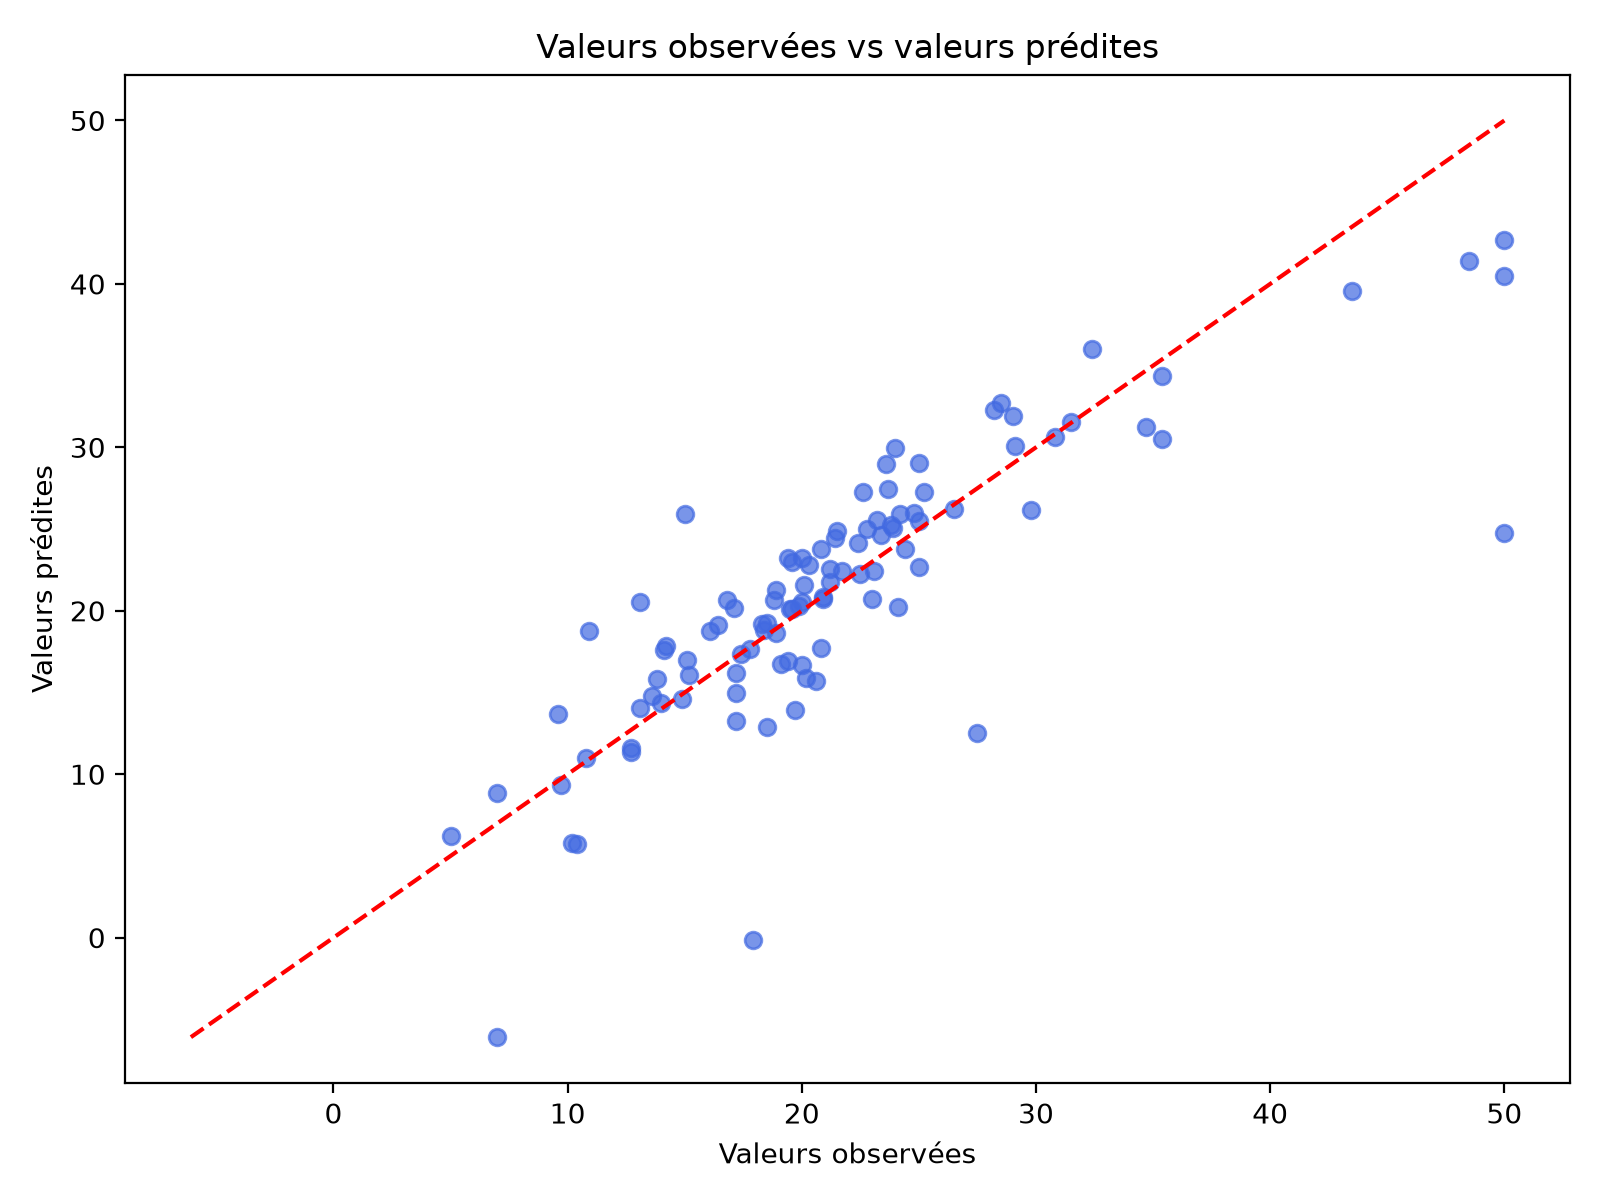
\includegraphics[width=0.85\textwidth]{images/predictions_vs_observed.png}
\caption{Valeurs observées vs valeurs prédites}
\end{figure}

\subsection{Interprétation des coefficients}
Les coefficients estimés mettent en évidence les variables les plus influentes. Parmi les variables les plus déterminantes, on observe notamment :

\begin{itemize}[leftmargin=1.5em]
    \item le nombre de pièces par logement : relation positive forte ;
    \item le pourcentage de population défavorisée : relation négative forte ;
    \item la distance aux centres d’emploi : relation négative ;
    \item le ratio élèves-professeurs : relation négative ;
    \item la présence de pollution atmosphérique : relation négative.
\end{itemize}

Les résultats sont cohérents avec l’intuition économique : des logements plus grands et mieux situés sont associés à des prix plus élevés, tandis que des quartiers moins favorisés ou plus pollués sont associés à des valeurs plus faibles.

\section{Vérification des hypothèses du modèle}

\subsection{Hétéroscédasticité}
Le diagramme des résidus par rapport aux prédictions montre une dispersion croissante à mesure que les prédictions augmentent. Le test de Breusch-Pagan confirme cette observation : la statistique vaut 59,189087 avec une p-value très faible, ce qui rejette l’hypothèse d’homoscédasticité. Les résidus ne sont donc pas homoscédastiques.

\begin{figure}[H]
\centering
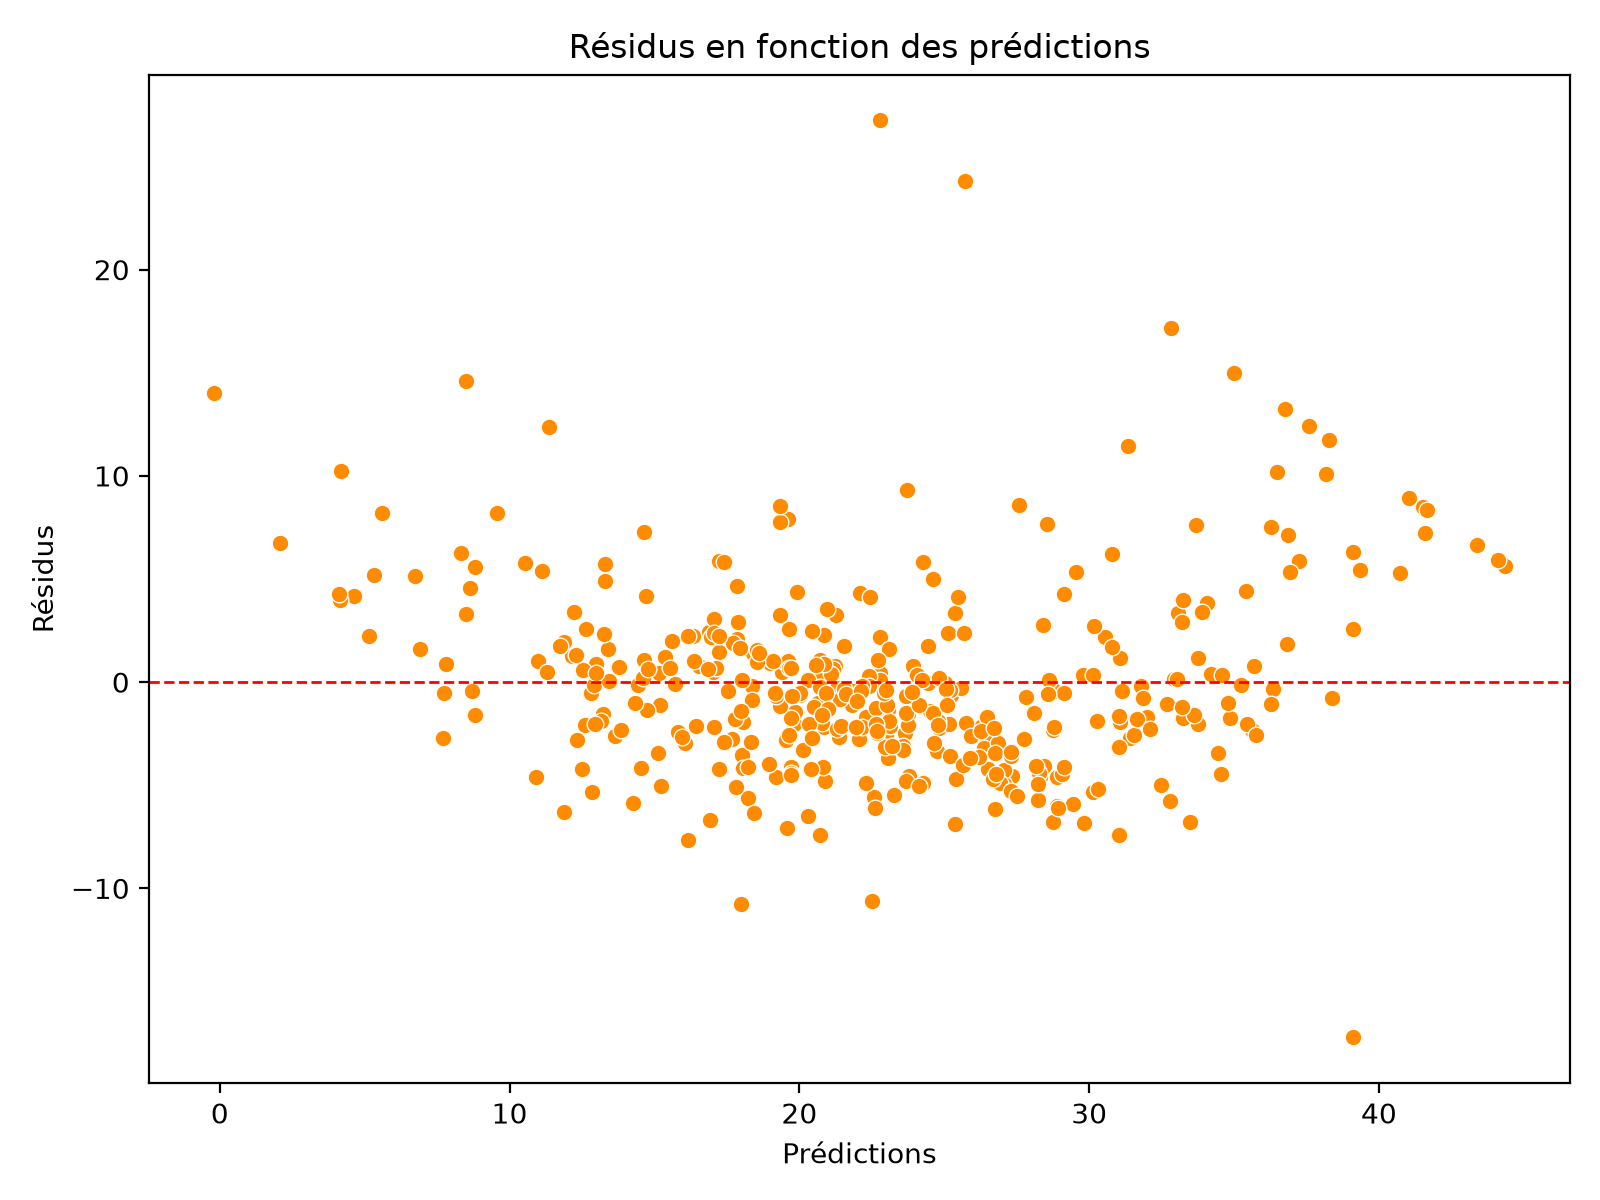
\includegraphics[width=0.85\textwidth]{images/residus_vs_predictions.png}
\caption{Résidus vs prédictions}
\end{figure}

\subsection{Normalité des résidus}
Les tests de normalité indiquent une déviation significative par rapport à une loi normale. Le test de Shapiro-Wilk, ainsi que le QQ-plot, montrent que les résidus ne suivent pas exactement une distribution gaussienne. La même conclusion ressort des tests de Kolmogorov-Smirnov et d’Anderson-Darling.

\begin{figure}[H]
\centering
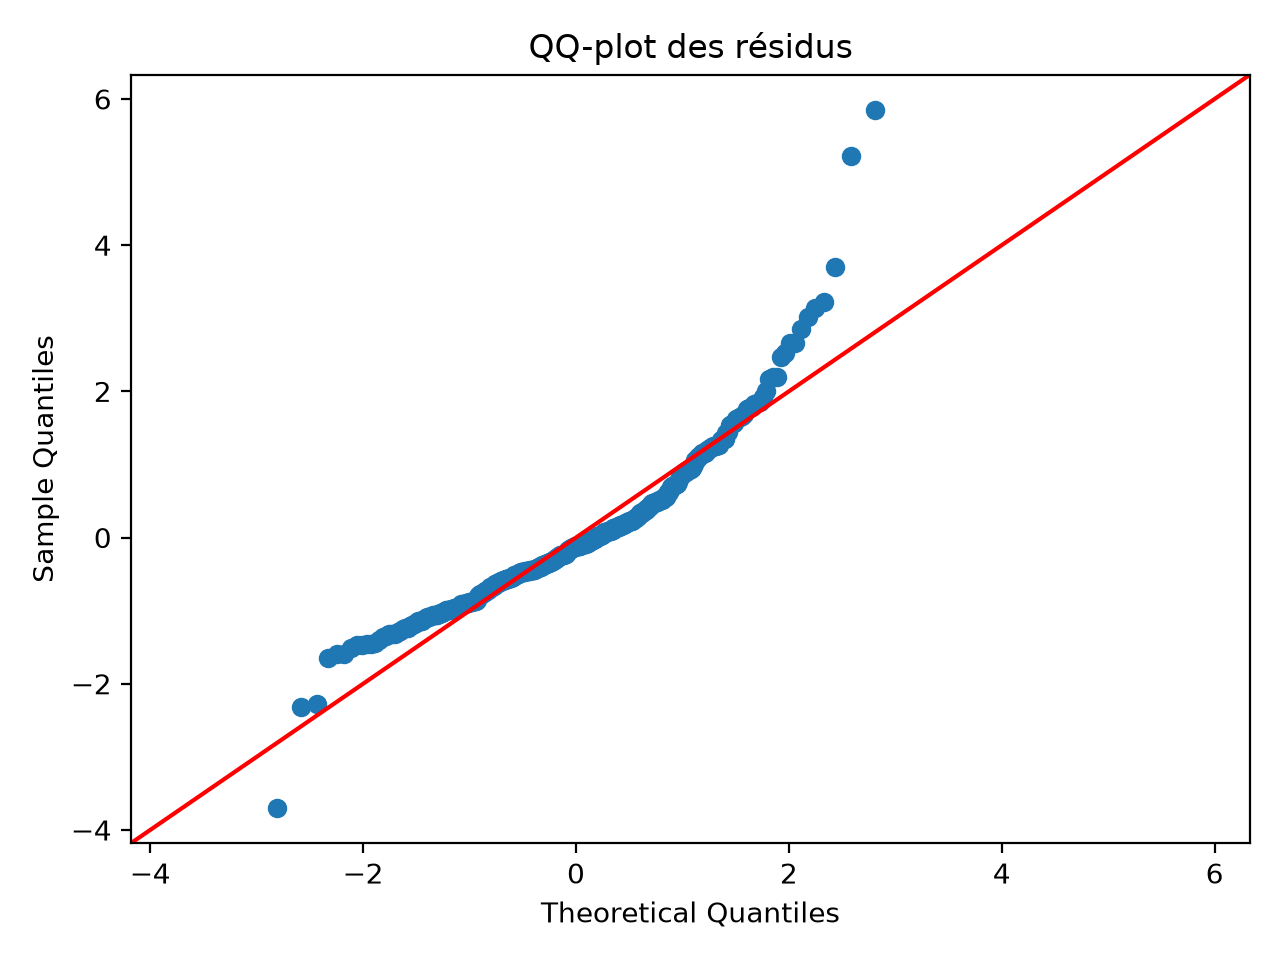
\includegraphics[width=0.8\textwidth]{images/qqplot_residus.png}
\caption{QQ-plot des résidus}
\end{figure}

\subsection{Autocorrélation et multicolinéarité}
Le test de Durbin-Watson est proche de 2, ce qui suggère l’absence de corrélation résiduelle forte. Concernant la multicolinéarité, les valeurs VIF restent globalement acceptables, bien qu’un niveau de vigilance soit conseillé pour certaines variables fortement corrélées entre elles.

\begin{table}[H]
\centering
\caption{Synthèse des diagnostics du modèle}
\begin{tabular}{p{4.5cm}p{2.8cm}p{5.5cm}}
\toprule
Diagnostic & Résultat & Interprétation \\
\midrule
Breusch-Pagan & p-value $< 10^{-6}$ & Hétéroscédasticité détectée \\
Durbin-Watson & 2.114123 & Pas de forte autocorrélation \\
Shapiro-Wilk & p-value $< 10^{-6}$ & Non-normalité des résidus \\
Anderson-Darling & fort écart & Non-normalité confirmée \\
Kolmogorov-Smirnov & p-value $< 10^{-6}$ & Distribution résiduelle non gaussienne \\
\bottomrule
\end{tabular}
\end{table}

\section{Discussion et limites}

Le modèle de régression linéaire reste pertinent pour ce projet car il est interprétable et simple à expliquer. Il permet de comprendre l’influence relative des principales variables sur la valeur des logements. Cela en fait un bon point de départ pédagogique et analytique.

Cependant, plusieurs limites doivent être soulignées. Les hypothèses de normalité et d’homoscédasticité ne sont pas entièrement satisfaites, ce qui limite l’interprétation stricte des tests de significativité et des intervalles de confiance. De plus, les relations entre certaines variables et la cible semblent non linéaires, en particulier pour le pourcentage de population défavorisée. Enfin, le jeu de données date de 1970 et ne reflète pas nécessairement le marché immobilier actuel.

Dans un travail ultérieur, il serait utile de tester des modèles plus avancés, tels qu’une régression régularisée, une régression log-linéaire ou un modèle non linéaire. On pourrait aussi utiliser une validation croisée pour stabiliser les performances et comparer plusieurs formulations du modèle.

\section{Conclusion}

Cette étude montre qu’une régression linéaire multiple permet d’expliquer une part substantielle de la variance du prix des logements à Boston. Avec un $R^2$ de 0,7509 sur l’entraînement et de 0,6688 sur le test, le modèle se révèle utile pour capturer les relations entre caractéristiques urbaines et valeur des logements. La baisse de performance entre entraînement et test reste modérée, ce qui laisse penser à une bonne capacité de généralisation.

Le projet a permis de mettre en pratique les étapes essentielles d’une analyse de données : préparation, exploration, modélisation, évaluation et diagnostic. Il a également démontré l’importance d’interpréter les résultats avec critique, car un modèle performant n’est pas forcément exempt de violations d’hypothèses. En ce sens, la régression linéaire constitue ici un bon point d’entrée dans le monde de la modélisation prédictive, tout en laissant place à des améliorations futures plus avancées.

\section{Références}
\begin{itemize}
    \item Harrison, D., et Rubinfeld, D. L. (1978). Hedonic housing prices and the demand for clean air. \textit{Journal of Environmental Economics and Management}. \\
    \item James, G., Witten, D., Hastie, T., et Tibshirani, R. (2013). \textit{An Introduction to Statistical Learning}. Springer. \\
    \item Documentation scikit-learn. \\
    \item Documentation statsmodels.
\end{itemize}

\end{document}
